\section{Numerical examples, reproducibility, and verification}

\subsection{The critical curves over the binary field}

Let $d=\binom n2-1$ and let $a$ be the number of observations beyond $d$.
The following values are evaluations of the proved limiting products, not fitted simulation curves.
The dimension-only total variation is the largest difference in acceptance probabilities achievable by a test that uses only $\dim N$.
With equal prior probabilities for the two models, its best success probability is $(1+T_2(a))/2$.

\begin{center}
\begin{tabular}{@{}rrr@{}}
\toprule
$a$ & Linear-recovery probability $F_2(a)$ & Dimension-test distance $T_2(a)$\\
\midrule
$-1$ & $0$ & $0.1925253967$\\
$0$ & $0.2887880951$ & $0.2887880951$\\
$1$ & $0.5775761902$ & $0.2887880951$\\
$2$ & $0.7701015869$ & $0.5775761902$\\
$3$ & $0.8801160993$ & $0.7701015869$\\
$4$ & $0.9387905059$ & $0.8801160993$\\
$5$ & $0.9690740706$ & $0.9387905059$\\
$6$ & $0.9844561987$ & $0.9690740706$\\
\bottomrule
\end{tabular}
\end{center}

The mean and variance of the limiting binary observation overhead are
\[
\mathbb EC_2=1.6066951524152917\ldots,
\qquad \operatorname{Var}(C_2)=2.744033888759488\ldots.
\]
For $q=3$, the corresponding values are $0.6821535026052381\ldots$ and
$0.9494332401401026\ldots$. The expectation result is dimension-independent in the limit: the unknown form has order $n^2$ coefficients, but the extra samples beyond $d$ have a bounded limiting mean.

\begin{figure}[htbp]
\centering
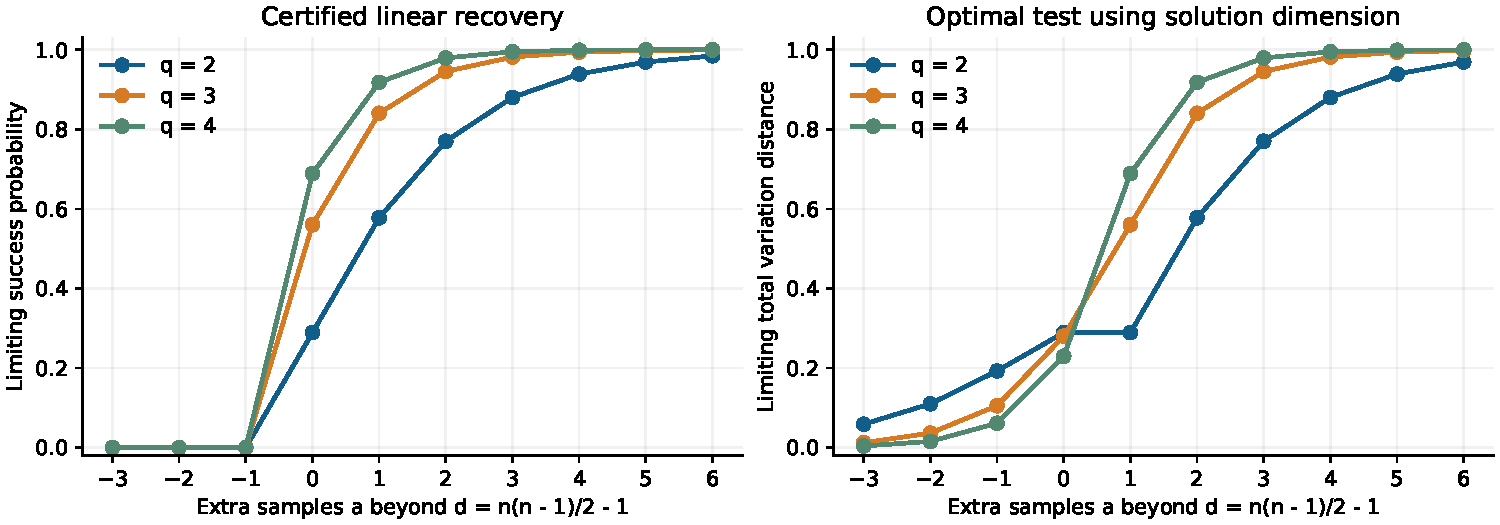
\includegraphics[width=\linewidth]{figures/critical_profiles.pdf}
\caption{Exact limiting profiles from Corollaries~\ref{crit:recovery} and~\ref{crit:testing}. The two panels concern different statistical tasks. The recovery algorithm certifies a one-dimensional solution space; the testing panel uses only its dimension.}
\label{fig:critical}
\end{figure}

\subsection{Independent exact checks}

The program \texttt{code/verify\_hidden\_forms.py} enumerates all two-planes and all alternating forms on $\mathbb F_2^4$ and $\mathbb F_3^4$. It computes incidences directly, separately from the theoretical Fourier formulas. There are respectively $35$ and $130$ two-planes, of which $15$ and $40$ are isotropic for the chosen nondegenerate form. The $64+729$ alternating forms give $2(64+729)=1586$ exact comparisons of the null and planted Fourier identities. All agree as rational numbers.

The same program computes complete finite-dimensional binary nullity laws by an exact dynamic program on row spaces, through $12$ observations for $n=4$. Its transition counts use the enumerated planes; it does not substitute the limiting iid law. These data provide small-dimensional examples, including a reminder that the asymptotic approximation need not be close when $n$ is small.

For numerical illustration, $5000$ independent trajectories in each of the null and planted models were generated at each of $n=6,10,14$, with seed $20261127$. The largest empirical distance from the limiting law over offsets $-2$ through $5$ was about $0.2032$ at $n=6$, $0.0124$ at $n=10$, and $0.0109$ at $n=14$. These are Monte Carlo comparisons containing both sampling error and finite-size effects; they are not proofs or deterministic error bounds. At the exact threshold $a=0$, the planted runs at $n=10$ gave $1435/5000=0.2870$ one-dimensional solution spaces, compared with the limit $0.2887880951\ldots$.

The products defining the plotted curves are truncated after $300$ factors. The elementary bound
\[
0\le1-\prod_{j>M}(1-q^{-j})\le\sum_{j>M}q^{-j}=\frac{q^{-M}}{q-1}
\]
controls this truncation. Standard double-precision rounding affects the printed last digits; the identities themselves are proved algebraically.

\subsection{The arithmetic decoder implementation}

The program \texttt{code/noisy\_path\_decoder.py} implements (NG4). It reads a real position array, the mesh, an optional position-error bound and a finite list of prime probes. Its default bandwidth is (NG11), with increment-error bound twice the supplied position-error bound. The chosen smooth window is
\[
w(v)=Z^{-1}\exp\!\left[-\frac1{(v-1)(2-v)}\right]\mathbf1_{(1,2)}(v),
\quad Z=\int_1^2\exp\!\left[-\frac1{(v-1)(2-v)}\right]dv,
\]
with $J_w\simeq1.96254112181544$. It reports the estimates, the asymptotic standard-deviation scale, and the two quantities in (NG9). It does not mislabel an asymptotic standard deviation as a finite-sample certified confidence interval.

The program \texttt{code/verify\_analytic\_algebra.py} checks the exact extrapolation identities for orders $1$ through $8$, including the allocation factor $(2^m-1)^2$. It also compares the decoder against a directly evaluated three-jump synthetic path to check the sign, angle inversion, and normalization. That synthetic path is not a Dirichlet Li--L\'evy path and supplies no empirical proof of the analytic theorem.

Floating-point evaluation is a practical illustration of the mathematical estimator. The theorem states separately how deterministic probe-evaluation errors enter the total error. A fully certified numerical implementation would need error-controlled transcendental evaluation and numerical upper bounds for the constants in (NG22). Neither is asserted by the included floating-point script.

\subsection{Rebuilding and the verification boundary}

The archive is self-contained for rebuilding the report. From its top directory run
\begin{verbatim}
pdflatex -interaction=nonstopmode -halt-on-error \
  finite_observation_and_critical_recovery.tex
pdflatex -interaction=nonstopmode -halt-on-error \
  finite_observation_and_critical_recovery.tex
python3 code/verify_hidden_forms.py --repetitions 5000
python3 code/verify_analytic_algebra.py
\end{verbatim}
The Python scripts use NumPy, SciPy and Matplotlib; their versions in the preparation environment are recorded in \texttt{results/environment.json}. The exact incidence checks and finite row-space enumeration use Python integers and rational arithmetic. JSON files retain the complete counts and numerical outputs.

The mathematical proofs were separately checked for source dependencies, generator-domain justification, adaptive-noise control, covariance scaling, low-rank exceptional sets, transition coupling, and stopping-time tails. The review corrected an initially proposed accelerated Gaussian assertion: the final higher-order theorem claims only the mean-square rates justified by its proof, while the sharp Gaussian theorem retains the narrower mesh conditions (NG9).

No new Lean proof is included. The artifact establishes its claims through the written proofs and supplemental finite checks. The upstream theorem's verification status is reported from its primary verification source, rather than inferred from these computations. Global novelty, growing-conductor statistical constants, the compatible nondegenerate-form count, and full-data optimal hidden-form testing remain outside the established conclusions.
